\documentclass[a4paper,11pt]{article}
\usepackage{fontspec}
\setmainfont{Noto Serif CJK SC}
\XeTeXlinebreaklocale "zh"
\XeTeXlinebreakskip=0pt plus 1pt
\usepackage[margin=25mm]{geometry}
\usepackage{graphicx}
\usepackage[backend=biber,style=numeric]{biblatex}
\addbibresource{references.bib}
\title{固定图形与文稿构建验收}
\author{Pi Research 技术验收}
\date{}
\begin{document}
\maketitle
\section*{范围与来源}
本文件用于隔离编译、中文显示和固定来源追溯的软件验收，不包含新的科学结论。
图形由上一批已批准容器实际生成，包含 21 个合成数据点。文稿引用自有验收协议\cite{acceptance}，该协议不是科学论文。
编译成功只证明此固定源文件集合能够产生 PDF，不替代科学审查。
\newpage
\section*{固定图形}
\begin{figure}[h]
\centering
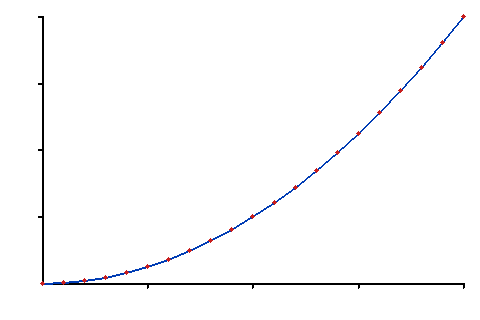
\includegraphics[width=0.8\linewidth]{figure.png}
\caption{固定 v1 图形：合成的平方关系示例，不代表真实科研测量。}
\end{figure}
\printbibliography
\end{document}
